% -------------------------------------------------------------------------------- %

\begin{exercise}

Zeigen Sie, dass für Funktionen $f$ von beschränkter Variation $\abs{\hat f(n)} \leq \frac{\sqrt 2}{\sqrt \pi n} \norm[\mathrm{BV}]{f}$, $n \neq 0$.

Hinw.:
Verwenden Sie partielle Integration für Riemann-Stieltjes-Integrale.

\end{exercise}

% -------------------------------------------------------------------------------- %

\begin{solution}

Wir gehen davon aus, dass $f: \T \to \R$.
Mit $\norm[\mathrm{BV}]{f}$ ist wahrscheinlich die Totalvariation $V_\T(f)$ von $f$ auf $\T$ gemeint.

\begin{tcolorbox}[standard jigsaw, opacityback = 0]
    \centering
    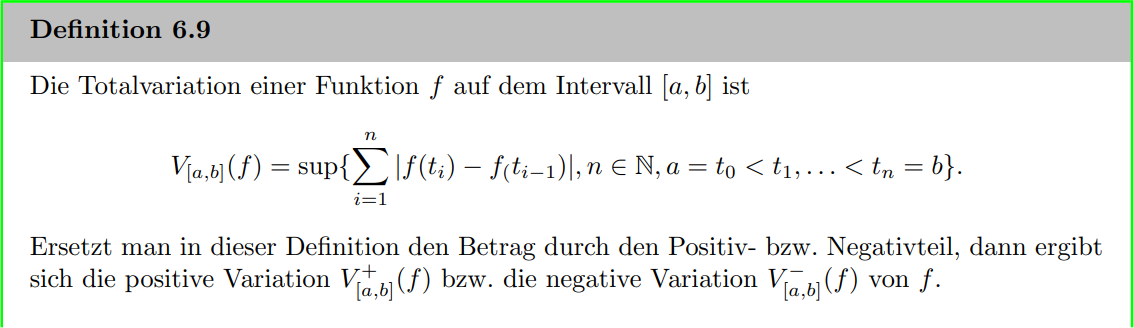
\includegraphics
    [width = 0.75 \textwidth]
    {MassWHT1&2/MassWHT1&2 - Definition 6.9.1.png} \\
    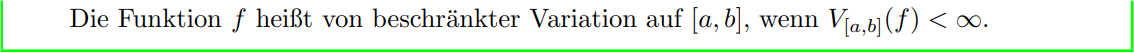
\includegraphics
    [width = 0.75 \textwidth]
    {MassWHT1&2/MassWHT1&2 - Definition 6.9.2.png}    
\end{tcolorbox}

Ein paar Sachen müssen wir über Riemann-Stieltjes-Integrale wissen.

\begin{enumerate}[label = \arabic*.]

    \item Sache (partielle Integration für Riemann-Stieltjes-Integrale):
    
    \begin{align*}
        \Int[a][b]{f}{g}
        =
        f(b) g(b)
        -
        f(a) g(a)
        -
        \Int[a][b]{g}{f}
    \end{align*}

    \item Sache:
    
    \includegraphicsboxed{Ana1&2/Ana1&2 - 11.2.5 Satz.png}

    \item Sache:
    
    \begin{align*}
        \Int[a][b]{f}{g}
        \leq
        \norm[\infty]{f}
        \norm[\mathrm{BV}]{g}
    \end{align*}

\end{enumerate}

Angeblich ist folgende Familie von Funktionen eine ONB von $L^2(\T)$.

\begin{align*}
    e_n(x)
    :=
    \frac{1}{\sqrt{2 \pi}}
    e^{i n x},
    \quad
    x \in \T,
    \quad
    n \in \Z
\end{align*}

Wir berechnen deren Stammfunktionen $\Forall n \in \Z, \Forall x \in \T:$

\begin{align*}
    E_n(x)
    :=
    \pbraces{\int e_n}(x)
    =
    \frac{1}{\sqrt{2 \pi}}
    \pbraces{\Int{e^{-i n t}}{t}}(x)
    =
    \frac{1}{\sqrt{2 \pi}}
    \frac{1}{-i n}
    e^{-i n x}
    =
    \frac{i}{\sqrt{2 \pi} n}
    e^{-i n x}.
\end{align*}

\begin{align*}
    \implies
    \Forall n \in Z:
    \norm[\infty]{E_n}
    =
    \sup_{x \in \T}
    \abs
    {
        \frac{i}{\sqrt{2 \pi} n}
        e^{-i n x}
    }
    =
    \frac{1}{\sqrt{2 \pi} n}
    \sup_{x \in \T}
    \abs{e^{-i n x}}
    =
    \frac{1}{\sqrt{2 \pi} n}    
    e^{-i n \pi}
    =
    \frac{1}{\sqrt{2 \pi} n}
\end{align*}

\begin{align*}
    \implies
    \abs{\hat f(n)}
    & =
    \abs
    {
        \frac{1}{\sqrt{2 \pi}}
        \Int[-\pi][\pi]
        {
            f(x) e^{-i n x}
        }{x}    
    }
    =
    \abs
    {
        \Int[-\pi][\pi]
        {
            f(x) e_n(x)
        }{x}
    }
    \stackrel
    {
        \text{$2$. Sache}
    }{=}
    \abs
    {
        \frac{1}{\sqrt{2 \pi}}
        \Int[-\pi][\pi]{f}{E_n}
    } \\
    & \stackrel
    {
        \text{$1$. Sache}~
        \mathrm{(PI)}
    }{=}
    \abs
    {
        f(x) E_n(x) \Big |_{x = -\pi}^\pi
        -
        \Int[-\pi][\pi]{E_n}{f}
    } \\
    & \leq
    \abs
    {
        f(\pi) \frac{i}{\sqrt{2 \pi} n} e^{-i n \pi}
        -
        f(-\pi) \frac{i}{\sqrt{2 \pi} n} e^{-i n \pi}
    }
    +
    \abs
    {
        \Int[-\pi][\pi]{E_n}{f}
    } \\
    & \leq
    \frac{1}{\sqrt{2 \pi} n} |f(\pi) - f(-\pi)|
    +
    \norm[\infty]{E_n}
    \norm[\mathrm{BV}]{f}
    \leq
    \frac{1}{\sqrt{2 \pi} n}
    \norm[\mathrm{BV}]{f}
    +
    \frac{1}{\sqrt{2 \pi} n}
    \norm[\mathrm{BV}]{f}
    =
    \frac{2}{\sqrt{2 \pi} n}
    \norm[\mathrm{BV}]{f} \\
    & =
    \frac{\sqrt 2}{\sqrt{\pi} n}
    \norm[\mathrm{BV}]{f}    
\end{align*}

\end{solution}

% -------------------------------------------------------------------------------- %
